% CVPR 2025 Paper Template; see https://github.com/cvpr-org/author-kit

\documentclass[10pt,twocolumn,letterpaper]{article}

%%%%%%%%% PAPER TYPE  - PLEASE UPDATE FOR FINAL VERSION
% \usepackage{cvpr}              % To produce the CAMERA-READY version
\usepackage{cvpr}      % To produce the REVIEW version
% \usepackage[pagenumbers]{cvpr} % To force page numbers, e.g. for an arXiv version

% Import additional packages in the preamble file, before hyperref
%
% --- inline annotations
%
\newcommand{\red}[1]{{\color{red}#1}}
\newcommand{\todo}[1]{{\color{red}#1}}
\newcommand{\TODO}[1]{\textbf{\color{red}[TODO: #1]}}
% --- disable by uncommenting  
% \renewcommand{\TODO}[1]{}
% \renewcommand{\todo}[1]{#1}

\usepackage{tabularx}
\usepackage{multirow}

\newcommand{\yearstartcuda}{2012}
\newcommand{\yearendcuda}{2024} % the present day

\newcommand{\yearstartddl}{2015}
\newcommand{\yearendddl}{2024} % the present day

%%%%%%%%%%%%%%%% Author specific packages
\usepackage[edges]{forest}

%%%%%%%%%%%%%%%% Define colors
\definecolor{hidden-black}{RGB}{20,68,106}
\definecolor{hidden-blue}{RGB}{194,232,247}


% Latex table
\usepackage{booktabs}
\usepackage{isotope}
\usepackage{siunitx}
\usepackage{makecell}

\sisetup{
 	per-mode = fraction, 
 	load-configurations = abbreviations,
}

% List in table
\newcommand{\tabitem}{~~\llap{\textbullet}~~}
\usepackage{longtable}
\usepackage{lipsum}  
\usepackage{enumitem}
\usepackage{graphicx}
\newcommand{\specialcell}[2][c]{%
  \begin{tabular}[#1]{@{}c@{}}#2\end{tabular}}


% References
\usepackage{nameref}
\usepackage{zref-user}

% Define a custom command for labeled sections
\newcommand{\cellref}[1]{%
  [\hyperref[#1]{#1}]%
}



% It is strongly recommended to use hyperref, especially for the review version.
% hyperref with option pagebackref eases the reviewers' job.
% Please disable hyperref *only* if you encounter grave issues, 
% e.g. with the file validation for the camera-ready version.
%
% If you comment hyperref and then uncomment it, you should delete *.aux before re-running LaTeX.
% (Or just hit 'q' on the first LaTeX run, let it finish, and you should be clear).
\definecolor{cvprblue}{rgb}{0.21,0.49,0.74}
\usepackage[pagebackref,breaklinks,colorlinks,allcolors=cvprblue]{hyperref}

%%%%%%%%% PAPER ID  - PLEASE UPDATE
\def\paperID{*****} % *** Enter the Paper ID here
\def\confName{CVPR}
\def\confYear{2025}

%%%%%%%%% TITLE - PLEASE UPDATE
\title{A Systematic Literature Review of Distributed Techniques for Parallelizing Stochastic Descent Backpropagation}

%%%%%%%%% AUTHORS - PLEASE UPDATE
\author{First Author\\
Department of Computer Science\\
University Name\\
{\tt\small firstauthor@university.edu}
\and
Second Author\\
Department of Computer Science\\
University Name\\
{\tt\small secondauthor@university.edu}}

\begin{document}
\maketitle
\begin{abstract}
	This paper presents a systematic literature review of distributed and parallel techniques for running
	deep neural networks on multiple machines and GPUs. It is composed of three parts: 1) a review of the
	available libraries that enable distributed training across GPU clusters, 2) a review of the
	most popular frameworks that facilitate parallelizing the training process on GPUs, and 3) a
	practical section that demonstrates a proof-of-concept implementation of the training process
	using common frameworks, namely PyTorch DDP and cuDNN.

	The review synthesizes research from the past decade, examining various approaches to distributed
	training, their effectiveness, and implementation challenges. The work is aimed at students and
	practitioners, with the goal to provide an introduction to the topic and help create a general idea
	of the most common libraries in each domain.

	The distributed experiments use data parallelism to accelerate the training process, while the GPU
	experiments use cuDNN, cuBLAS and manual kernel implementations to train a small network. The
	effectiveness of each approach is demonstrated and to aid reproduction and experimentation Docker
	environments are provided. This allows to simulate a multi-GPU setup on a single NVidia GPU, promoting
	ease of use by not relying on cloud services. The repository is available at 
	\url{https://github.com/atomwalk12/deep-bridge-survey}.
\end{abstract}

% Due to its many applications across various fields of research, engineering, and daily life, deep learning has seen a surge in popularity. Therefore, larger and more expressive models have been proposed, with examples like Turing-NLG using as many as 17 billion parameters. Training these very large models becomes increasingly difficult due to the high computational costs and large memory footprint. Therefore, several approaches for distributed training based on data parallelism (e.g., Horovod) and model/pipeline parallelism (e.g., GPipe, PipeDream) have emerged.  In this work, we focus on an in-depth comparison of three different parallelism models that address these needs: data, model and pipeline parallelism.

% Because training a deep neural network (DNN) takes arduous amounts of time and computation, often researchers expedite the training process via distributed parallel training on GPUs.
% On one hand, this lower computing-to-communication ratio makes traditional data parallelism difficult to scale, and traditional model parallelism leads to low GPU utilization. Both make it difficult to obtain a higher speedup. On the other hand, multi-GPU systems exhibit complex connectivity among GPUs.

% Experiments with four different DNN models show that Pipetorch averages 1.4x speedup compared to data parallelism. 

% TODO Razvan: explain model, data, pipeline and hybrid parallelism.

%  We demonstrate FCUBE executing five different learners contributed by three different machine learning groups on a 100 node deployment on Amazon EC2. They collectively solve a publicly available classification problem trained with 11 million exemplars from the Higgs dataset.     

% Step 1: Getting started
% - Goals, expected outputs, constraints, search terms and keywords
% ===== STEP 1: Getting Started =====
% This section covers:
% - Goals and expected outputs
% - Initial constraints
% - Search terms and keywords
\section{Introduction}
\label{sec:intro}

\subsection{Background}
Machine learning (ML) has become essential for extracting knowledge from data across diverse
applications. Deep learning, a subfield of ML using artificial neural networks, is increasingly
important, especially with the massive amounts of data now available
\cite{ben-nun_demystifying_2020}, \cite{dehghani_distributed_2023}, \cite{langer_distributed_2020}.
Distributed deep learning (DDL) has become crucial due to the increasing size of datasets and model
complexity \cite{berloco_systematic_2022}, \cite{dehghani_distributed_2023}. This literature review
focuses on the core concepts, techniques, and frameworks used to implement and optimise DDL.
Challenges in scaling deep learning include distributing ML programs, bridging computation with
communication, and determining what to communicate between machines \cite{xing_strategies_2015}.
This systematic review will provide a comprehensive overview of the current state of DDL and
address these questions, identify gaps, and give direction for future research
\cite{langer_distributed_2020}, \cite{ben-nun_demystifying_2020}, \cite{dehghani_distributed_2023},
\cite{verbraeken_survey_2021} \TODO{Review citations}.

\subsection{Importance of the Topic}
\label{sec:importance_of_topic}
The increasing volume of data necessitates advanced analysis techniques, making distributed deep
learning essential. Efficiently training deep learning models is vital for research and development
\cite{dehghani_distributed_2023}, \cite{chahal_hitchhikers_2018}, \cite{xing_strategies_2015}. This
review is important for both practitioners and researchers, providing an overview of techniques and
frameworks for implementing DDL solutions \cite{dehghani_distributed_2023},
\cite{berloco_systematic_2022} and also highlighting current research trends and future
opportunities \cite{berloco_systematic_2022}, \cite{ben-nun_demystifying_2020}. This review
addresses gaps in existing surveys by focusing on practical implementation and a detailed analysis
of the performance and efficiency of different DDL techniques \cite{berloco_systematic_2022}
\TODO{review citation}. The outcomes of this review will aid software engineers in selecting and
implementing appropriate DDL techniques.

\subsection{Research Questions}
\label{sec:research_questions}
This review addresses the following research questions. Below are listed the key questions concerning DDL:

\begin{itemize}
	\item What are the different techniques for parallelising deep learning models and data
	      \cite{berloco_systematic_2022, ben-nun_demystifying_2020, langer_distributed_2020}?
	      % NOTE \item How do parameter update strategies impact distributed deep learning systems (e.g., Parameter Server and decentralised approaches) \cite{ben-nun_demystifying_2020,berloco_systematic_2022,langer_distributed_2020}?
	\item How is stochastic gradient descent (SGD) computed in distributed environments
	      \cite{berloco_systematic_2022,ben-nun_demystifying_2020,langer_distributed_2020,verbraeken_survey_2021}? % NOTE and what are the associated challenges 
	\item What are the key frameworks currently available for implementing DDL, and how do their features
	      compare \cite{berloco_systematic_2022}?
\end{itemize}

Concerning GPU parallelization, the following questions are of interest: \TODO{Could be improved}
\begin{itemize}
	\item How does CUDA enable data parallelization on single-machine GPUs?
	\item What are key frameworks for implementing CUDA parallelization?
	\item What similarities are there between CUDA and DDL techniques?
\end{itemize}

Of particular interest is to check for intertwined connections between the two topics:
\begin{itemize}
	\item In what ways are the techniques used in DDL also useful in GPU parallelization?
\end{itemize}

% TODO Razvan
% \begin{enumerate}
%     \item What distributed techniques have been developed for parallelizing stochastic descent backpropagation?
%     \begin{itemize}
%         \item How does CUDA enable data parallelization on single-machine GPUs?
%         \item What methods are available for parallelizing learning across PC clusters, particularly using PyTorch's DDP?
%     \end{itemize}

%     \item How do these techniques compare in terms of convergence speed and computational efficiency?
%     \begin{itemize}
%         \item What are the performance differences between CUDA-based GPU implementations and CPU-only approaches?
%         \item How does data parallelization scale in GPU clusters, and what are its limitations?
%     \end{itemize}

%     \item What are the primary challenges and solutions in implementing distributed training systems?
%     \begin{itemize}
%         \item What are the key considerations when implementing cluster parallelization using DDP?
%         \item How can data parallelization be effectively implemented on GPUs using CUDA?
%     \end{itemize}
% \end{enumerate}

\subsection{Scope and Methodology}
% First introduce the workflow
This systematic review follows a rigorous methodology outlined in Figure \ref{fig:workflow}. The
workflow consists of seven main steps, starting with getting started (Step 1), through to the final
wrap-up of the report (Step 7). Reproducibility and transparency of the review process is a
priority. As a result multiple artifacts will be produced at each phase. These artifacts are
reported separately in the appendix.

\TODO{Too many subsections}

% TODO Razvan
% Our investigation includes practical implementations and experimental work:
% \begin{itemize}
%     \item Cluster parallelization demonstrations using PyTorch's DDP module
%     \item GPU implementations with CUDA, including:
%     \begin{itemize}
%         \item Code examples showing data parallelization on GPUs
%         \item Comparative implementations using CPUs
%         \item Performance analysis and benchmarking
%     \end{itemize}
% \end{itemize}

\subsection{Paper Organization}
The remainder of this paper is organized as follows: Section \ref{sec:protocol} presents our
systematic review protocol including the study selection framework and search process
documentation, Section \ref{sec:methods} describes our systematic review methodology, including the
search strategy across digital libraries, inclusion/exclusion criteria, and quality assessment
protocol. Section \ref{sec:results} presents our findings, Section \ref{sec:discussion} discusses
the implications, and Section \ref{sec:conclusion} concludes with future research directions. This
structure ensures a logical flow from background to findings and recommendations.


% Step 2: Define search strategy & 
% Step 3: Selection of relevant studies
% ===== STEP 2: Define Search Strategy =====
% This section covers:
% - Search strategy development
% - Documentation of search process

\begin{figure*}[th]
	\centering
	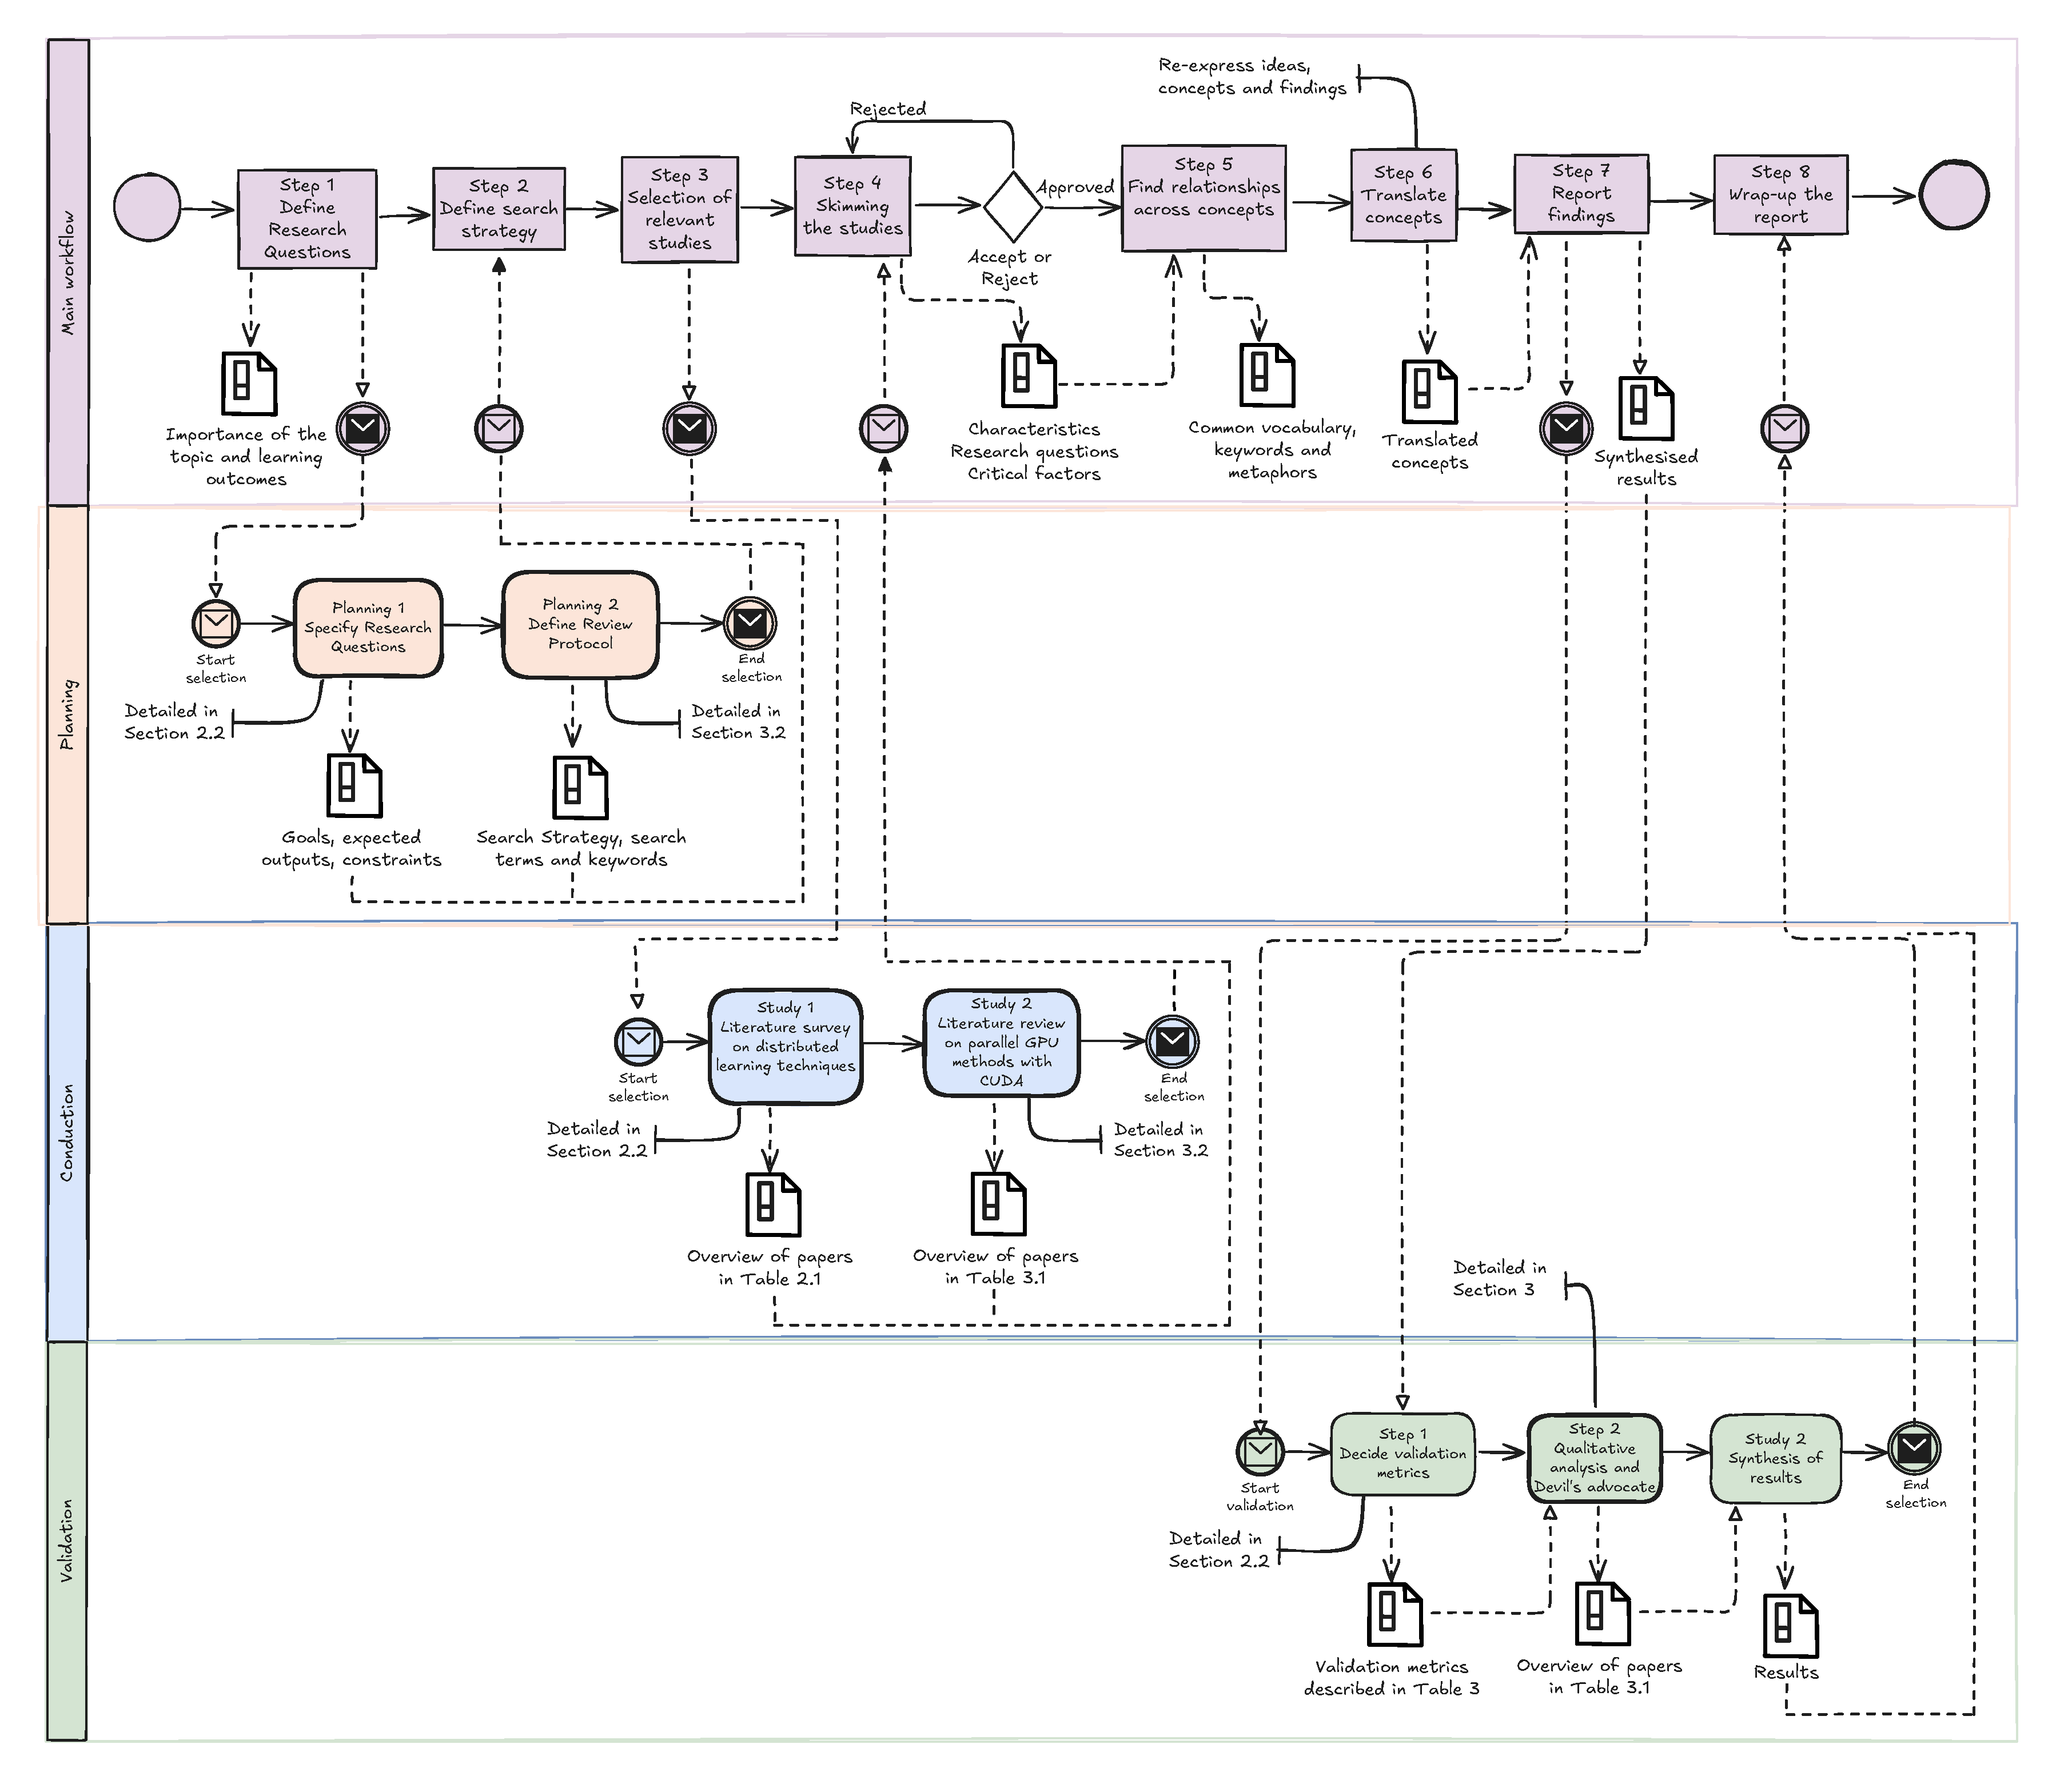
\includegraphics[width=\linewidth]{figures/workflow2}
	\caption{Systematic review workflow showing the main steps, documentation artifacts, and validation processes.
		The workflow is divided into three main phases: main workflow (top), studies selection (middle), and
		validation (bottom). Dashed lines indicate documentation and communication flows. Adapted from \cite{dos_santos_sustainable_2024}.}
	\label{fig:workflow}
\end{figure*}

\section{Related Work}
\label{sec:related_work}

\TODO{Reference the related work on survying the present methods both in DDL and CUDA}

Related work focuses on techniques and algorithms for training deep learning models across multiple
machines \cite{dehghani_distributed_2023, chahal_hitchhikers_2018, berloco_systematic_2022}. These
sources explore various aspects of DDL, such as parallelization techniques and communication
methods. However, our contribution emphasizes the connection between DDL and GPU programming with
CUDA. Furthermore, this study details the main libraries for DDL and GPU programming. We will also
provide practical guidance on running a small neural network in CUDA and facilitating PyTorch
Distributed Data Parallel (DDP) programming using Docker, addressing a practical implementation gap
not covered in the previous work. \TODO{Highlight related surveys concerning CUDA}

This study follows primarily the guidelines described in \cite{keele_systematic_2007}, however
advice for conducting the review is synthesized from a wider range of related articles
\cite{brereton_lessons_2007-1,kitchenham_procedures_nodate,budgen_reporting_2018,dos_santos_sustainable_2024}.

Distributed training of neural networks has become essential for modern deep learning applications
due to increasing model complexity and dataset sizes \cite{chahal_hitchhikers_2018}. The main
approaches for distributing neural network training can be categorized into several key strategies
\cite{dehghani_distributed_2023}:

\begin{itemize}
	\item \textbf{Data Parallelism:}
	      The dataset is divided across multiple nodes, with each node training a complete copy of the
	      model on its portion of data. Gradients from all nodes are then combined to update the model parameters.
	      This approach can be implemented either synchronously (all nodes wait for each other) or asynchronously (nodes work independently).

	\item \textbf{Model Parallelism:}
	      The neural network model itself is divided across different nodes, with each node responsible
	      for computing a specific portion of the model architecture. This strategy is particularly useful
	      when the model is too large to fit on a single machine.

	\item \textbf{Pipeline Parallelism:}
	      The training process is divided into sequential stages, similar to an assembly line,
	      where the output of one stage becomes the input for the next. This allows different parts
	      of the model to train simultaneously while maintaining dependencies.

	\item \textbf{Hybrid Parallelism:}
	      This approach combines multiple parallelization strategies to optimize training efficiency.
	      For example, model parallelism might be used to distribute a large model across GPUs, while
	      data parallelism is applied to each model segment.
\end{itemize}

These approaches can be further enhanced through techniques such as gradient compression, mixed
precision training, and tensor fusion \cite{dehghani_distributed_2023}. The choice of specific
techniques depends on factors including model architecture, available hardware, and training
requirements. For a comprehensive review of these techniques and their implementations, readers are
referred to \cite{chahal_hitchhikers_2018}.

\section{Research method}
\label{sec:protocol}

Multiple studies in the literature emphasize that a literature survey should be both transparent
and replicable \cite{keele_systematic_2007, dos_santos_sustainable_2024-1}, the main reason being
that this allows to minimize reviewer bias. This is a valid concern in general, however especially
so in this survey since it is conducted by only one person. In a broader study, bias would normally
be minimized by having multiple iterations with more than one reviewer involved. In this paper,
steps have been taken to mitigate this bias, acknowledging that it is not possible to eliminate it
completely. To ensure this, the process is documented and most of the resulting artifacts are
present in the text and in the Appendix. Moreover, AI classifiers were used during the screening
process to make the selection manageable by one person. The details are provided in Section
\ref{sec:ai-screening}.

% TODO these are all good but was hoping to minimize the number of citations
% TODO \cite{keele_systematic_2007,brereton_lessons_2007-1,budgen_reporting_2018, dos_santos_sustainable_2024-1},

% Now detail Step 1 content
The workflow is shown in Figure \ref{fig:workflow} where the key phases are annotated as follows:
Getting Started (M.1, M.2), Planning the Review (M.3, M.4), Conducting the Review (M.5, M.6), and
Reporting the Review (M.7, M.8). M.2 calls an auxiliary process composed of S.1 and S.2 to select
the appropriate studies \TODO{add references across the paper}.

\subsection{M.1 -- The need for a survey}
\label{sec:need_for_survey}

\textbf{Importance of the topic.}
Distributed techniques are important in neural networks because they allow models with billions of
parameters to perform a large number of computations in a reasonable amount of time. One of the
pioneering papers in machine learning that made use of GPUs to train neural networks in parallel
(AlexNet \cite{krizhevsky_imagenet_2012}), mentioned that the network took "between five and six days to
train on two GTX 580 3GB GPUs", suggesting that the training time would have taken much longer on a
CPU.

One key property of distributing neural network architectures to a larger number of parameters, is
that one can achieve better generalization and lower error rates even when training on smaller
datasets \cite{kaplan_scaling_2020}. This gives the impression of intelligence due to the model's
ability to make predictions that seem insightful. Understanding innate details on how these
libraries function, can provides a fertile foundation for future ideas.

\textbf{Learning outcomes.}
As a result of conducting the survey I expect the following learning outcomes: learn from the primary
studies, improve writing and research skills, gain practical experimental expertise using CUDA and
Pytorch DDP and identify potential research ideas for future projects.

\subsection{M.2 -- Getting started}
\label{sec:research_questions}
Building on the learning outcomes defined in Section \ref{sec:need_for_survey}, we define
the goals, expected outputs and constraints. The main goal was to analyze parallelization frameworks in DDL and CUDA.
The expected results were to identify key frameworks for each category. For this, we defined two main constraints: (i)
we only considered frameworks that introduce CUDA and DDL frameworks and (ii) we included only primary
studies that were peer-reviewed, although literature surveys were used to gain familiarity with the topic,
however they are only discussed in Section \ref{sec:related_work}. These ideas are formally defined
in Section \TODO{...} and \TODO{...}.

\subsection{M.3 -- Selection of Relevant Studies}
This step identified and selected studies from both areas (CUDA programming and DDL). I collected
studies of the state of the art of both CUDA frameworks (in Step S.1) and DDL libraries (in Step
S.2).

\subsubsection{S.1 -- Survey on CUDA programming libraries}
\paragraph{S.1.1 -- Problem definition.}
In order to identify interesting frameworks and broaden the understanding of the topic, I conducted
a secondary study\footnote{A secondary study synthesizes primary papers to provide a comprehensive
	overview. This contrasts with tertiary studies which analyze secondary studies.}. This decision was
made in the problem definition step (S.1.1 in Figure \ref{fig:workflow-study}). In order to do this
systematically, this section defines a research protocol during the planning phase, which is then
used to find related studies. The research protocol is essentially a framework for conducting the
review. This section outlines the key decisions that were made with to create the protocol by
identifying the research questions and search strategy.

\begin{figure*}[th]
	\centering
	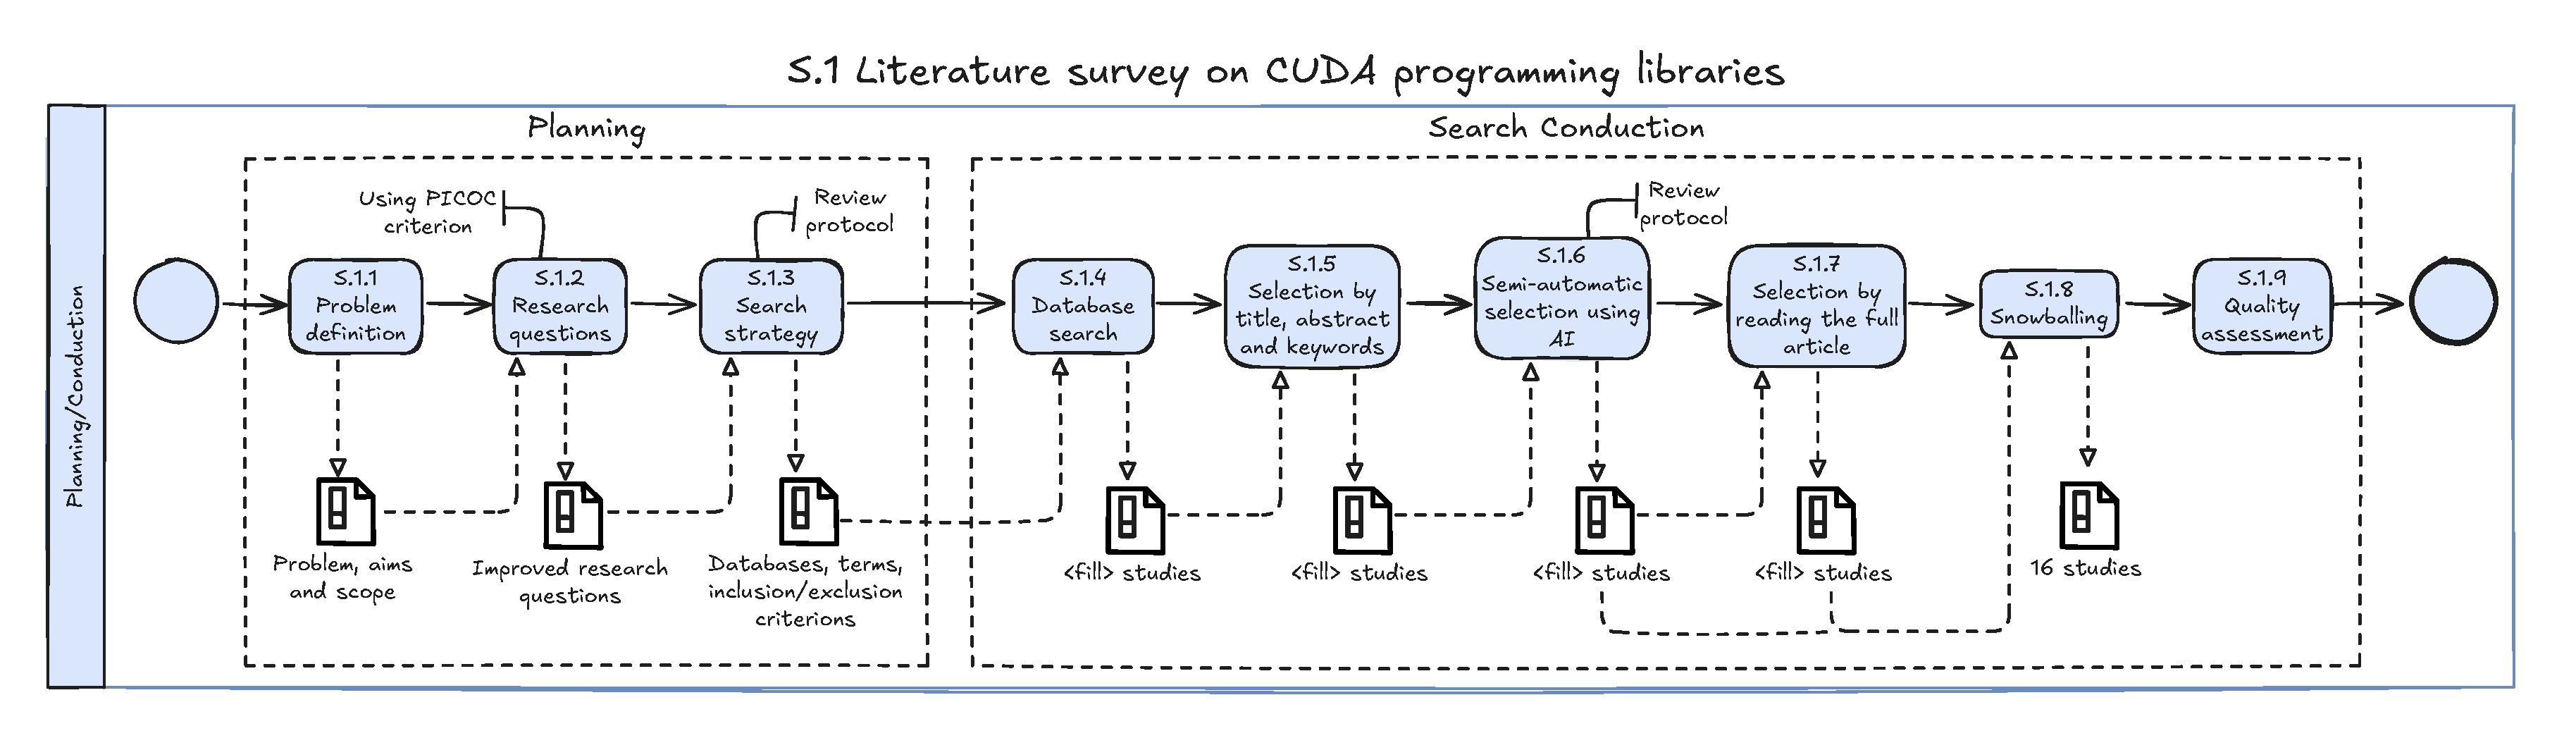
\includegraphics[width=\linewidth]{figures/workflow3}
	\caption{The diagram suggests the key steps for finding papers related to the CUDA programming survey. The phases
		include planning the review (aims, research questions, search strategy) and conducting the review (study selection phase). The research questions
		were transformed according to the PICOC (Population, Intervention, Comparison, Outcome, Context) criterion suggested by \cite{keele_systematic_2007}.}.
	\label{fig:workflow-study}
\end{figure*}

\paragraph{S.1.2 -- Research questions.}
After an initial literature review, the research questions (RQ) defined in Section
\ref{sec:initial_research_questions} are refined using the guidelines defined in
\cite{kitchenham_evidence-based_2015} and \cite{keele_systematic_2007}. Specifically, the PICOC
(Population, Intervention, Comparison, Outcome, Context) criterion is used to transform the
questions into a format that ensures them to be specific, measurable and well-defined. The
questions below are ordered based on their significance in the survey:

% TODO: remove this
% \begin{itemize}
% 	\item \textbf{RQ\textsubscript{1}} What are the most common frameworks currently available for 
% 		  GPU programming with CUDA, and how do their usability compare?
% 		  % NOTE implementing distributed deep learning, and how does their usability compare?
% 	      % NOTE \cite{berloco_systematic_2022, ben-nun_demystifying_2020, langer_distributed_2020}?
% 	      % NOTE \item How do parameter update strategies impact distributed deep learning systems (e.g., Parameter Server and decentralised approaches) \cite{ben-nun_demystifying_2020,berloco_systematic_2022,langer_distributed_2020}?
% 	\item How is stochastic gradient descent (SGD) computed in distributed environments
% 	      \cite{berloco_systematic_2022,ben-nun_demystifying_2020,langer_distributed_2020,verbraeken_survey_2021}? % NOTE and what are the associated challenges 
% 	\item What are the key frameworks currently available for implementing DDL, and how do their features 
% 	      compare \cite{berloco_systematic_2022}?
%  	\item In what ways are the techniques used in DDL also useful in GPU parallelization?
% \end{itemize}

% TODO: \TODO{RQ1: ease of learning, ease of use and documentation compare?}

\begin{itemize}
	\item \textbf{RQ\textsubscript{1}:} In the field of Deep Learning, what are the most frequently cited
	      frameworks for GPU programming using CUDA, and how do their user communities differ in size? \\
	      \textit{Rationale:} By identifying the most common frameworks, we can identify which are the gaps
	      in the literature they cover and which are the most promising areas for future research.

	\item \textbf{RQ\textsubscript{2}:} In the field of Deep Learning, what are the most commonly cited
	      frameworks for distributed training of neural networks across clusters, and how do their respective user communities vary in size? \\
	      \textit{Rationale:} By identifying the most common frameworks, we can trace the years in which they were published
	      and form a unified timeline of the evolution of the field with respect to the related CUDA programming advancements.

	      % NOTE Razvan I am conducting a literature review in the field of deep learning, specifically focusing on distributed training of 
	      % NOTE neural networks across clusters. I need to identify the most commonly cited frameworks used for this purpose.
	\item \textbf{RQ\textsubscript{3}:} What practical applications of these technologies have been reported in the literature? \\
	      \textit{Rationale:} This can yield hands-on experience on the topic which is helpful for practical applications.
	\item \textbf{RQ\textsubscript{4}:} What are the overlaps in data/model optimization strategies used in DDL and GPU parallelization? \\
	      \textit{Rationale:} By identifying the overlaps, it offers a more unified view of how the concepts are interrelated.
\end{itemize}

The questions play a key role in guiding the search strategy, data extraction process and results
synthesis phase.

\paragraph{S.1.3 -- Search Strategy.}
The search strategy represents represents a systematic approach for identifying relevant studies
that adequately answer the research questions.

\paragraph{Databases.}
The process involves a manual search of four citation databases --
\href{https://ieeexplore.ieee.org/}{IEEE Xplore}, \href{https://dl.acm.org/}{ACM Digital Library},
\href{https://www.sciencedirect.com/}{Science Direct}, and \href{https://www.scopus.com/}{Scopus}
-- that include conference proceedings and journal papers, considering three metadata fields
(title, abstract, and keywords).

\paragraph{Inclusion/Exclusion Criteria.}
There were defined four inclusion criteria (IC) and three exclusion criteria (EC). In particular, I
decided to select only primary studies, however secondary studies were mentioned in Section
\ref{sec:related_work}. The identification of secondary studies was useful since the selected
studies synthesize evidence and can make it possible to access primary studies:

\begin{itemize}
	\item \textbf{IC\textsubscript{1}}: Study is a primary study and is peer-reviewed.
	\item \textbf{IC\textsubscript{2}}: Study addresses distributed frameworks in DL.
	\item \textbf{IC\textsubscript{3}}: Study addresses GPU programming with CUDA.
	\item \textbf{IC\textsubscript{4}}: Study introduces a library or a framework. \\
	\item \textbf{EC\textsubscript{1}}: Study does not discuss implementation details.
	\item \textbf{EC\textsubscript{2}}: Study is not a primary study.
	\item \textbf{EC\textsubscript{3}}: Study is not written in English.
\end{itemize}

\paragraph{Search terms.}
In Step S.1.3, I inquired about the literature using the following search string:
\begin{quote}
	\textit{( "machine learning" OR "deep learning" )
		AND
		( "Data parallelism" OR "model parallelism")
		AND
		( "framework" OR "implementation" )}
\end{quote}

While in Step S.2.3, the following search string was used \TODO{review string}:
\begin{quote}
	\textit{( "machine learning" OR "deep learning" )
		AND
		( "Data parallelism" OR "model parallelism")
		AND
		( "framework" OR "implementation" )}
\end{quote}

The details and justification to define this search string can be found in the supplementary
material in Section \ref{sec:search_strategy}.

\paragraph{Publication year criteria.}
The search was restricted to papers published between $\yearstartcuda$-$\yearendcuda$ for the CUDA
task and $\yearstartddl$-$\yearendddl$ for the DDL task. The former start year ($\yearstartcuda$)
was chosen as the baseline due to being the year when AlexNet \cite{krizhevsky_imagenet_2012} was
published. This paper revolutionized research in neural networks by allowing advanced AI models to
be trained on GPUs.

The latter start year ($\yearstartddl$) was chosen as at this point there was a shift towards
resource conservation, which resulted in a focus on concurrency within mini-batches
\cite{ben-nun_demystifying_2020}. This is the year by which the effectiveness of deep learning
algorithms was more widely recognized and more research was published that focused on scalability.

\paragraph{S1.4 - S1.5 -- Study selection}
After an initial database search (Step S1.4), \todo{fill-me} studies were retrieved. A selection
process was initiated by reading the title, abstract and keywords of each study (S.1.5), resulting
in \todo{fill-me} studies.

\paragraph{S1.6. -- Semi-automatic selection using AI}
\label{sec:ai-screening}
Next, as suggested in \cite{brereton_lessons_2007-1}, I applied
AI inference engines to filter resulting studies into a more easily digestible set (S.1.6). The technique
is semi-automatic with a focus on screening and extraction of relevant information.

\begin{table}[htbp]
	\centering
	\caption{The Search Engines Used in this Survey}
	\label{tab:databases}
	\begin{tabular}{llllr}
		\hline
		ID & Tool           & Stage  & Mode    & Number of uses \\
		\hline
		1  & IEEExplore     & Search & Web     & 33             \\
		2  & ACM            & Search & Web     & 30             \\
		3  & ScienceDirect  & Search & Web     & 24             \\
		4  & Web of Science & Search & Web     & 19             \\
		5  & Google Scholar & Search & Web     & 18             \\
		6  & SpringerLink   & Search & Web     & 17             \\
		7  & Scopus         & Search & Web     & 14             \\
		8  & Compendex      & Search & Desktop & 11             \\
		9  & CiteSeer       & Search & Web     & 5              \\
		\hline
	\end{tabular}
\end{table}

\begin{table}[htbp]
	\centering
	\caption{\footnotesize Number of studies before and after applying the IC and EC}
	\label{tab:criteria}
	\begin{tabular}{lrrrrr}
		\hline
		                           & \footnotesize IEEE   & \footnotesize Science & \footnotesize Scopus & \footnotesize ACM     & \footnotesize Total \\
		                           & \footnotesize Xplore & \footnotesize Direct  &                      & \footnotesize Library &                     \\
		\hline
		\footnotesize Before IC/EC & 22                   & 10                    & 10                   & 30                    & 72                  \\
		\footnotesize After IC/EC  & 10                   & 10                    & 10                   & 30                    & 60                  \\
		\hline
	\end{tabular}
\end{table}

% ===== STEP 3: Selection of Relevant Studies =====
% This section details:
% - Study 1: Distributed learning techniques
% - Study 2: CUDA implementations

% Combined "Purpose," "Scope," and "Relationship Between Study Types"
This section defines the aims and scope of the review, clarifying the types of studies to be
included and the rationale for exploring distributed learning and CUDA implementations together.
The specific objectives of the review are aligned with the associated research questions to provide
a clear focus. The boundaries of the review concern the types of distributed learning techniques
and CUDA implementations considered, with a time period between 2015 and 2022 to ensure currency.
The review includes studies focusing on the design and analysis of distributed learning algorithms
and those focusing on CUDA-based parallel implementations to understand the translation of
theoretical aspects into practical implementations. This approach allows for the exploration of
patterns and challenges in mapping distributed algorithms onto parallel architectures
\TODO{Different topics explored together}.

\subsubsection{Distributed Learning Techniques Review}
The review will focus on distributed learning approaches, aligning with "Study 1" in Figure
\ref{fig:workflow}, with the following considerations:
\begin{itemize}
	\item Types of algorithms including \textbf{data parallelism, model parallelism, and asynchronous
		      Stochastic Gradient Descent (SGD)} \cite{ben-nun_demystifying_2020,langer_distributed_2020}.
	\item Different distributed architectures including parameter servers and peer-to-peer systems
	      \cite{verbraeken_survey_2021,ben-nun_demystifying_2020,langer_distributed_2020}.
	\item Specific machine learning models such as neural networks and support vector machines.
\end{itemize}

\subsubsection{CUDA-based Parallel Implementation Review}
For CUDA implementations, the review will consider aspects relevant to "Study 2" in Figure
\ref{fig:workflow}:
\begin{itemize}
	\item Implementation of distributed methods on NVIDIA GPUs using the CUDA framework
	\item Different CUDA libraries and architectures
	\item Specific hardware considerations including GPUs and Tensor Processing Units (TPUs)
\end{itemize}

\subsubsection{Justification for Inclusion}
Both distributed learning techniques and CUDA implementation studies will be included to provide a
complete picture of the current state-of-the-art research in the area. By including both study
types, a deeper understanding of both theoretical approaches and implementation techniques for
practical applications can be reached.

\subsection{Preliminary Protocol Development}
This systematic review follows the guidelines proposed by Kitchenham and Charters for software
engineering research. The preliminary review protocol was developed to establish the foundation for
the steps visualized in Figure \ref{fig:workflow}, particularly in the initial stages. An overview
of the papers included after the initial selection phase (corresponding to the output of the
"Studies Selection" phase in Figure \ref{fig:workflow}) will be presented in Table 2.1.

\subsubsection{Background and Rationale}
This section provides the necessary context for the review, outlining the research gaps that will
be addressed \cite{ben-nun_demystifying_2020}. It explicitly states the need for a systematic
review of the current literature to address this gap and provide a focused analysis.

\subsubsection{Initial Search Strategy}
The initial search strategy involves combining keywords using Boolean and proximity operators to
generate search strings, based on the "Goals, expected outputs, constraints, search terms and
keywords" documented as an input to Step 1 in Figure \ref{fig:workflow}. Databases like Scopus,
Google Scholar, and ACM Digital Library are selected for their coverage of computer science,
engineering, and applied mathematics literature. Studies published between 2015-2022 will be
considered to ensure recent advancements are included while maintaining a consistent period for
analysis.
\begin{itemize}
	\item \textbf{Search Terms:} Details of the search terms will be provided in Section \ref{sec:search_process_documentation}.
	\item \textbf{Database Justification:} Rationale for selecting specific databases is detailed in Section \ref{sec:search_process_documentation}.
	\item \textbf{Timeline:} The timeframe for including studies is 2015-2022.
\end{itemize}

\subsubsection{Preliminary Selection Criteria}
Preliminary criteria for inclusion will use specific examples such as ``studies that evaluate the
performance of synchronous distributed SGD in deep learning models'' rather than general terms like
``distributed computing'' \cite{ben-nun_demystifying_2020}. Preliminary quality thresholds will
ensure only high-quality studies are included in the final analysis. Specific inclusion and
exclusion criteria are detailed in Section \ref{sec:study-selection-criteria}.

\subsubsection{Initial Data Extraction Plan}
The following information will be extracted from each study:
\begin{itemize}
	\item Details of distributed systems \cite{ben-nun_demystifying_2020,langer_distributed_2020}:
	      \begin{enumerate}
		      \item Number of nodes
		      \item Communication network
		      \item Communication method
		      \item Topology
	      \end{enumerate}
	\item Machine learning algorithms and models used \cite{xing_strategies_2015}.
	\item Datasets and benchmarks \cite{ben-nun_demystifying_2020}.
	\item Performance metrics (training time, accuracy, speedup)
	      \cite{ben-nun_demystifying_2020,langer_distributed_2020,xing_strategies_2015}.
	\item CUDA implementation details (libraries, optimizations)
	      \cite{verbraeken_survey_2021,ben-nun_demystifying_2020,xing_strategies_2015}.
\end{itemize}
Further details on the data extraction strategy can be found in Section \ref{sec:data-extraction-strategy}.

\subsubsection{Quality Assessment Framework}
Preliminary quality assessment will use specific criteria to evaluate the validity and reliability
of methods, using established checklists from the literature \cite{ben-nun_demystifying_2020}. A
Likert scale will be used for a standardized approach. Detailed guidelines for reviewers will be
established to ensure consistency and prevent bias, as described further in Section
\ref{sec:quality-assessment-process}.
\begin{itemize}
	\item \textbf{Criteria:} Specific criteria are detailed in Section \ref{sec:quality-assessment-process}.
	\item \textbf{Scoring System:} A Likert scale will be used.
	\item \textbf{Guidelines:} Guidelines for reviewers are detailed in Section \ref{sec:quality-assessment-process}.
\end{itemize}

\subsubsection{Synthesis Approach}
The synthesis approach will involve meta-analysis where appropriate, using statistical analysis to
combine results from included studies with clearly defined methods
\cite{ben-nun_demystifying_2020}. Thematic synthesis will be used for narrative synthesis, allowing
an in-depth understanding of themes present in selected studies.
\begin{itemize}
	\item \textbf{Meta-analysis:} Details of the methods will be defined later.
	\item \textbf{Narrative synthesis:} Thematic synthesis will be employed.
\end{itemize}

\subsection{Search Process Documentation}
\label{sec:search_process_documentation}
This section provides an overview of our search strategy. Detailed search documentation, including exact search strings and results for each database, can be found in the supplementary materials (Section \ref{sec:search_strategy}).

\subsubsection{Search Strategy Overview}
Our search strategy combines terms from two main categories as shown in Table
\ref{tab:search_terms}. The number of articles retrieved from each database is presented in Table
\ref{tab:search_results}.

\begin{table*}[ht]
	\centering
	\caption{Number of Retrieved Articles by Database}
	\label{tab:search_results}
	\begin{tabular}{|l|c|c|c|}
		\hline
		\textbf{Database}   & \textbf{Initial Results} & \textbf{After Filtering} & \textbf{Final Selection} \\
		\hline
		Scopus              & XXX                      & XXX                      & XXX                      \\
		\hline
		Google Scholar      & XXX                      & XXX                      & XXX                      \\
		\hline
		ACM Digital Library & XXX                      & XXX                      & XXX                      \\
		\hline
		IEEE Xplore         & XXX                      & XXX                      & XXX                      \\
		\hline
		Science Direct      & XXX                      & XXX                      & XXX                      \\
		\hline
		arXiv               & XXX                      & XXX                      & XXX                      \\
		\hline
		\textbf{Total}      & XXX                      & XXX                      & XXX                      \\
		\hline
	\end{tabular}
\end{table*}

The complete search strings for each database, including any database-specific adaptations, are
documented in Section \ref{sec:search_strategy} of the supplementary materials.

\subsection{Study Selection Criteria}
\label{sec:study-selection-criteria}
This section specifies the detailed inclusion and exclusion criteria for the studies to be included
in the review. These will be specific, measurable, and objective to ensure that all studies are
assessed consistently and fairly \cite{ben-nun_demystifying_2020}.

% TODO: Razvan. Is this fine?
\subsubsection{Inclusion Criteria}
The following criteria will be used for including studies:
\begin{itemize}
	\item Studies published between 2013 and 2023
	\item Peer-reviewed articles and high-quality preprints
	\item Studies focusing on distributed training techniques
	\item Articles written in English
	\item Implementation details available
\end{itemize}
\cite{verbraeken_survey_2021,ben-nun_demystifying_2020}.

\subsubsection{Exclusion Criteria}
Studies will be excluded based on the following criteria:
\begin{itemize}
	\item Studies not focused on neural network training
	\item Pure theoretical papers without implementation
	\item Secondary studies (surveys, reviews)
	\item Insufficient technical details or results
\end{itemize}

\subsection{Quality Assessment Process}
\label{sec:quality-assessment-process}
This part of the methodology details the process used to assess the quality of the selected studies, aligning with the "Validation" phase shown in the bottom section of Figure \ref{fig:workflow}.

\subsubsection{Quality Criteria}
The quality of the studies will be evaluated based on the methodological rigour, clarity of
reporting, limitations of the studies, and potential for bias. Established checklists, such as
those provided by the CASP, will be used to address bias and validity in a rigorous and systematic
way.

\subsection{Data Extraction Strategy}
\label{sec:data-extraction-strategy}
This section details how data will be extracted from the included studies. The data extraction form will be designed to capture all necessary information, including study details, methodology, implementation specifics, dataset details, and results. The form will be piloted to ensure it captures the information effectively \cite{ben-nun_demystifying_2020}.

% \subsubsection{Extraction Form}
% The data extraction form was iteratively refined through:

% TODO Razvan
% \begin{itemize}
%     \item Publication metadata
%     \begin{itemize}
%         \item Authors, venue, year
%         \item Citation count and impact
%     \end{itemize}
%     \item Technical details
%     \begin{itemize}
%         \item Distributed training approach
%         \item Implementation specifications
%         \item Hardware configurations
%     \end{itemize}
%     \item Performance metrics
%     \begin{itemize}
%         \item Training time and convergence
%         \item Resource utilization
%         \item Scalability measures
%     \end{itemize}
%     \item Experimental setup
%     \begin{itemize}
%         \item Dataset characteristics
%         \item Hardware specifications
%         \item Software frameworks used
%     \end{itemize}
% \end{itemize}

\begin{itemize}
	\item \textbf{Details:} The data extraction form will capture study design, participants, interventions, and outcomes, as well as details of the implementation in distributed systems and parallel CUDA frameworks \cite{ben-nun_demystifying_2020}.
	\item \textbf{Piloting:} The extraction form will be piloted to ensure effectiveness \cite{ben-nun_demystifying_2020}.
	\item \textbf{Study Details:} The form will capture relevant details including implementation specifics.
\end{itemize}

% Final paragraph about methodology
By using this methodology, the systematic review will aim to provide a comprehensive and reliable
analysis of the current state of research in distributed deep learning and CUDA implementations.
The approach used here will enable the review to identify any trends and gaps in current research
and make recommendations for future study.

\subsection{Study Selection Results}
\label{sec:study_selection_results}
The complete lists of included and excluded studies, along with detailed information about each study, can be found in the supplementary materials (Section \ref{sec:study_selection}). A total of XXX studies were initially identified, with XXX studies meeting our inclusion criteria after screening. Table \ref{tab:study_types} provides an overview of the types of studies included in our review.

\begin{table*}[ht]
	\centering
	\caption{Overview of Included Study Types}
	\label{tab:study_types}
	\begin{tabular}{|l|c|p{8cm}|}
		\hline
		\textbf{Study Type}    & \textbf{Count} & \textbf{Description}                                                     \\
		\hline
		Empirical Studies      & XXX            & Studies with experimental evaluations of distributed learning techniques \\
		\hline
		Implementation Studies & XXX            & Studies focusing on CUDA implementations and optimizations               \\
		\hline
		Hybrid Studies         & XXX            & Studies covering both theoretical and implementation aspects             \\
		\hline
		\textbf{Total}         & XXX            &                                                                          \\
		\hline
	\end{tabular}
\end{table*}

\begin{itemize}
	\item \textbf{Goals:}
	\item To analyze parallelization frameworks in DDL.
	\item To evaluate libraries that support CUDA programming.
	\item To find out how these concepts are intertwined.
	\item To get practical experience with popular frameworks. \\
	\item \textbf{Expected Outputs:}
	\item Experience for conducting a systematic review.
	\item Systematic mapping of programming frameworks.
	\item Comparative analysis with strengths and weaknesses.
	\item Identification of research gaps. \\
	\item \textbf{Constraints:}
	\item Time period limited to 2012-2024\footnote{CUDA: 2012 is the year when AlexNet was published.} and
	      2015-2024\footnote{DDL: 2015 is the year when the shift towards scalability was noticed.}.
	\item Peer-reviewed articles and conference papers only.
	\item English language publications only.
	\item Technical implementation details must be present. \\
	\item \textbf{Search Terms and Keywords:}
	\item Listed in Table \ref{tab:search_terms}.
\end{itemize}

\begin{table*}[htbp]
	\centering
	\caption{The DNN papers included in the review}
	\label{tab:dnn_papers}
	\begin{tabular}{llp{8.01cm}p{2cm}lll}
		\hline
		\textbf{\#} & \textbf{Ref.}           & \textbf{Title}                                                                & \textbf{Type} & \textbf{Year} & \textbf{Citations} & \textbf{Stars}                             \\
		\hline
		1           & \cite{huang_gpipe_2019} & GPipe: Efficient Training of Giant Neural Networks using Pipeline Parallelism & Pipeline      & 2018          & 1446               & 2.8k \cite{noauthor_tensorflowlingvo_2025} \\
		2           & \cite{chen_mxnet_2015}  & MXNet: A Flexible and Efficient Machine Learning Library for Heterogeneous Distributed Systems & Hybrid (Data, Model) & 2015 & 2212 & 20.8k \cite{noauthor_apachemxnet_2025} \\
		3           & \cite{li_pytorch_2020}  & PyTorch Distributed: Experiences on Accelerating Data Parallel Training & Data & 2020 & 175 & 86.1k \cite{noauthor_pytorchpytorch_nodate} \\
		4           & \cite{xie_optimal_2022} & Optimal distributed parallel algorithms for deep learning framework Tensorflow & Hybrid (Data, Model) & 2022 & 10 & 187k \cite{abadi_tensorflow_2015} \\
		5           & \cite{rasley_deepspeed_2020} & DeepSpeed: System Optimizations Enable Training Deep Learning Models with Over 100 Billion Parameters & Hybrid (Data, Model) & 2020 & 1059 & 36.3k \cite{noauthor_microsoftdeepspeed_2025} \\
		6           & \cite{sergeev_horovod_2018} & Horovod: fast and easy distributed deep learning in TensorFlow & Data & 2018 & 1152 & 14.3k \cite{noauthor_horovodhorovod_2025} \\
		\hline
		% Add more papers as needed
	\end{tabular}
\end{table*}

% Step 4: Skimming the studies
% Details of Study 1: Literature survey on distributed learning techniques
% Details of Study 2: Literature review on parallel GPU methods with CUDA
%% ===== STEP 4: Skimming the Studies =====
% This section covers:
% - Initial screening process
% - Detailed in Section 2.2.1 (Study 1)
% - Detailed in Section 3.2 (Study 2)
\section{Methods}
\label{sec:methods}

% PLACEHOLDER: Study Selection Process
\TODO{PLACEHOLDER: Study Selection Process}
\subsection{Study Selection Process}
\subsubsection{Initial Screening}
Papers were initially screened based on:
\begin{itemize}
    \item Title and abstract relevance
    \item Citation count and venue quality
    \item Implementation details availability
\end{itemize}

% PLACEHOLDER: Study 1 Details
\TODO{PLACEHOLDER: Study 1 Details}
\subsection{Distributed Learning Analysis}
\subsubsection{Selection Criteria}
\begin{itemize}
    \item Clear description of distributed architecture
    \item Empirical performance measurements
    \item Scalability analysis
    \item Comparison with baseline methods
\end{itemize}

% PLACEHOLDER: Study 2 Details
\TODO{PLACEHOLDER: Study 2 Details}
\subsection{CUDA Implementation Analysis}
\subsubsection{Selection Criteria}
\begin{itemize}
    \item Detailed CUDA implementation description
    \item Performance benchmarks
    \item Memory usage analysis
    \item Optimization techniques
\end{itemize}

\TODO{Placeholder-end}



% Step 5: Find relationships across concepts
% Step 6: Translate concepts
% Step 7: Synthesize findings
%% ===== STEP 5: Find Relationships Across Concepts =====
% This section covers:
% - Common vocabulary and keywords
% - Relationships between studies
\section{Results}
\label{sec:results}

\subsection{Study Selection Results}
\begin{figure}[t]
    \centering
    \fbox{\rule{0pt}{2in} \rule{0.9\linewidth}{0pt}}
    \caption{PRISMA flow diagram showing the study selection process}
    \label{fig:prisma}
\end{figure}

\subsection{Quality Assessment Results}
[Quality assessment results will be presented here]

\subsection{Data Synthesis}
\subsubsection{Distribution Strategies}
[Discussion of different distribution strategies]

\subsubsection{Performance Analysis}
[Analysis of performance metrics]

\subsubsection{Implementation Challenges}
[Discussion of common implementation challenges]

\TODO{PLACEHOLDER: Cross-Study Analysis}
% PLACEHOLDER: Cross-Study Analysis
\subsection{Cross-Study Relationships}
\subsubsection{Common Patterns}
\begin{itemize}
    \item Communication bottlenecks
    \item Synchronization strategies
    \item Memory management techniques
    \item Performance optimization approaches
\end{itemize}

% ===== STEP 6: Translate Concepts =====
% This section maps:
% - Concepts between distributed and GPU implementations
% - Common patterns and terminology
\subsection{Concept Translation}
\label{sec:concept_translation}
\TODO{PLACEHOLDER: Concept Translation}

\subsubsection{Mapping Between Paradigms}
\begin{itemize}
    \item Node communication → CUDA streams
    \item Work distribution → Grid/Block organization
    \item Memory hierarchy → GPU memory types
    \item Load balancing → Kernel optimization
\end{itemize}

\subsubsection{Common Terminology and Patterns}
\begin{itemize}
    \item Parallelization strategies across both domains
    \item Synchronization mechanisms and their equivalents
    \item Memory management approaches
    \item Performance optimization techniques
\end{itemize}

\subsubsection{Implementation Mappings}
\begin{itemize}
    \item DDP concepts → CUDA implementations
    \item Cluster communication patterns → GPU memory patterns
    \item Resource allocation strategies → GPU resource management
    \item Error handling and recovery mechanisms
\end{itemize}
\TODO{Placeholder-end}

% Step 7: Synthesize findings (continued)
% - Re-express ideas, concepts and findings
%% ===== STEP 7: Synthesize Findings =====
% This section covers:
% - Re-express ideas, concepts and findings
% - Integration of both studies
\section{Discussion}
\label{sec:discussion}

% PLACEHOLDER: Synthesis of Studies
\TODO{PLACEHOLDER: Synthesis of Studies}
\subsection{Integration of Approaches}
\subsubsection{Complementary Aspects}
\begin{itemize}
    \item Combining distributed training with GPU acceleration
    \item Trade-offs between communication and computation
    \item Hybrid approaches for large-scale deployment
    \item Optimization strategies across scales
\end{itemize}

\subsection{Key Findings Synthesis}
\subsubsection{Common Themes}
\begin{itemize}
    \item Scalability challenges in both approaches
    \item Impact of hardware architecture
    \item Importance of efficient memory management
    \item Balance between parallelism and overhead
\end{itemize}

\subsection{Practical Applications}
\begin{itemize}
    \item Guidelines for implementation choices
    \item Best practices for hybrid systems
    \item Performance optimization strategies
    \item Resource allocation recommendations
\end{itemize}
\TODO{Placeholder-end}

\subsection{Interpretation of Findings}
Our systematic review answers the research questions posed in Section \ref{sec:research_questions} and reveals several key patterns in distributed training approaches:
\begin{itemize}
    \item Data parallelism remains the dominant paradigm for distributed training
    \item Communication overhead is a critical bottleneck in most implementations
    \item Synchronous approaches generally provide better convergence guarantees
    \item Asynchronous methods offer better scaling but with potential accuracy trade-offs
\end{itemize}

\subsection{Implications}
\subsubsection{Theoretical Implications}
The findings suggest several theoretical implications:
\begin{itemize}
    \item Need for better theoretical understanding of convergence in asynchronous settings
    \item Importance of communication-computation trade-offs
    \item Role of batch size in distributed training
\end{itemize}

\subsubsection{Practical Implications}
For practitioners, our review suggests:
\begin{itemize}
    \item Guidelines for choosing between synchronous and asynchronous approaches
    \item Best practices for implementing distributed training systems
    \item Common pitfalls and their solutions
\end{itemize}

\subsection{Limitations}
This review has several limitations:
\begin{itemize}
    \item Focus on published literature may miss industrial implementations
    \item Rapid pace of development in the field
    \item Limited access to implementation details in some studies
    \item Potential publication bias towards successful approaches
\end{itemize}

\subsection{Future Research Directions}
Based on our analysis, we identify several promising directions for future research:
\begin{enumerate}
    \item Development of adaptive communication strategies
    \item Integration of federated learning approaches
    \item Improved fault tolerance mechanisms
    \item Novel compression techniques for gradient communication
\end{enumerate} 
 
% Step 7: Wrap-up the report
%% ===== STEP 7: Wrap-up the Report =====
% This section covers:
% - Final synthesis
% - Future directions
% - Recommendations
\section{Conclusion}
\label{sec:conclusion}

\subsection{Summary of Findings}
This systematic review has examined the landscape of distributed techniques for parallelizing stochastic descent backpropagation. Our analysis of [X] primary studies reveals:
\begin{itemize}
    \item The evolution of distributed training approaches over the past decade
    \item Current best practices and their theoretical foundations
    \item Key challenges and proposed solutions
    \item Emerging trends and future directions
\end{itemize}

\subsection{Recommendations}
Based on our findings, we recommend:
\begin{enumerate}
    \item Careful consideration of communication patterns in distributed implementations
    \item Integration of modern compression techniques
    \item Adoption of hybrid approaches when appropriate
    \item Investment in robust monitoring and debugging tools
\end{enumerate}

\subsection{Main Challenges and Future Research Directions}
...


% PLACEHOLDER: Final Synthesis
\TODO{PLACEHOLDER: Final Synthesis}
\subsection{Comprehensive Overview}
Our systematic review has revealed several key insights:
\begin{itemize}
    \item The complementary nature of distributed and GPU-based approaches
    \item Critical factors for successful implementation
    \item Common challenges and solutions
    \item Emerging trends in both domains
\end{itemize}

\subsection{Future Research Directions}
Based on our analysis, we identify several promising areas:
\begin{enumerate}
    \item Integration of distributed and GPU-based approaches
    \item Novel synchronization strategies
    \item Advanced memory management techniques
    \item Automated optimization frameworks
\end{enumerate}

\subsection{Recommendations for Practice}
Key recommendations include:
\begin{itemize}
    \item Systematic approach to architecture selection
    \item Careful consideration of hardware constraints
    \item Implementation of monitoring and debugging tools
    \item Regular evaluation of system performance
\end{itemize}
\TODO{Placeholder-end}

\subsection{Final Remarks}
The field of distributed neural network training continues to evolve rapidly. While significant progress has been made in addressing key challenges, several important research questions remain open. Future work should focus on developing more efficient and scalable solutions while maintaining training stability and convergence guarantees. 



{
    \footnotesize
    \bibliographystyle{ieeenat_fullname}
    \bibliography{main}
}

% Supplementary material including:
% - Detailed validation metrics (Table 3)
% - Overview of papers (Table 2.1, Table 3.1)
% - Additional documentation
\clearpage
\setcounter{page}{1}
\maketitlesupplementary

\section{Supplementary Materials}
\label{sec:supplementary}

\subsection{Detailed Search Strategy}
\label{sec:search_strategy}

\subsubsection{Search Documentation}


A number of search strings were constructed using relevant terms deduced from the research. The
initial search strings are shown in the Appendix in Table \ref{tab:search_terms}. These terms are
combined in Table \ref{tab:search_documentation}, using boolean operators to generate query
strings, which are then used to search each individual database.

\begin{table*}[htbp!]
    \centering
    \caption{Core Search Terms for Distributed Deep Learning and GPU Programming}
    \label{tab:search_terms}
    \begin{tabularx}{\textwidth}{|l|X|X|}
        \hline
        \textbf{Category} & \textbf{Distributed Learning} & \textbf{GPU Computing} \\
        \hline
        Core Terms & 
        \textbf{"Distributed Deep Learning"},
        \textbf{"Parallel Deep Learning"},
        "Large-Scale Deep Learning" &
        \textbf{"GPU Programming"},
        \textbf{"CUDA Programming"} \\
        \hline
        Technical Approach & 
        \textbf{"Data Parallelism"},
        \textbf{"Model Parallelism"},
        \textbf{"Hybrid Parallelism"} &
        \textbf{"CUDA"},
        "GPU Optimization",
        "Parallel Computing" \\
        \hline
        Implementation & 
        \textbf{"Parameter Server"},
        \textbf{"All-Reduce"},
        \textbf{"SGD"} &
        \textbf{"CUDA Toolkit"},
        \textbf{"cuDNN"},
        "Multi-GPU" \\
        \hline
        Frameworks & 
        "TensorFlow",
        "PyTorch",
        "Horovod" &
        "TensorRT",
        "PyCUDA",
        "Numba" \\
        \hline
    \end{tabularx}
    \caption*{Note: Bold terms indicate primary search terms that will be prioritized.}
\end{table*}

The starting date used for the analysis starts from 2014 till 2024. The reason for utilizing this range
is due to the publishing date of \cite{SierraCanto2010ParallelTO}, which acts as a key paper in the domain. As a result,
I'd like to analyze the advancement of the field starting from this age. The key The following table 
documents our complete search process:

\begin{table*}[htbp!]
    \centering
    \caption{Detailed Search Documentation}
    \label{tab:search_documentation}
    \begin{tabularx}{\textwidth}{|l|X|c|c|c|}
        \hline
        \textbf{Database} & \textbf{Search String} & \textbf{Years Covered} & \textbf{Results} & \textbf{Filtered} \\
        \hline
        Scopus & ("Distributed Deep Learning" OR "Parallel Deep Learning") AND "Data Parallelism" & 2017-2024 & 82 & 11 \\
               & ( "machine learning" OR "deep learning" ) AND ( "Data parallelism" OR "model parallelism" OR "pipeline parallelism" OR "hybrid parallelism" ) AND ( "framework" OR "implementation" ) & 2012-2024 & 206 & 11 \\
        \hline
        ACM Digital Library & ("GPU Programming" OR "GPGPU Programming") AND ("CUDA" OR "CUDA Programming") AND ("Parallel Computing") & 2015-2022 & 2024-05-10 & 210 \\
        \hline
        Science Direct & [Exact search string] & 2015-2022 & 2024-05-10 & XXX \\
        \hline
        arXiv & [Exact search string] & 2015-2022 & 2024-05-10 & XXX \\
        \hline
    \end{tabularx}
\end{table*}


\subsubsection{Search Process Details}
\begin{itemize}
    \item \textbf{Years Covered:} 2015-2022
    \item \textbf{Language Restrictions:} English only
    \item \textbf{Document Types:} Journal articles, conference papers, and high-quality preprints
\end{itemize}

\subsubsection{Manual Searches}
The following additional sources were manually searched:
\begin{itemize}
    \item Key conference proceedings (e.g., NeurIPS, ICLR, ICML)
    \item Reference lists of included studies (snowballing)
    \item Citations of included studies (forward snowballing)
\end{itemize}

\subsection{Study Selection Details}
\label{sec:study_selection}

\subsubsection{Included Studies}
Table \ref{tab:included_studies} lists all studies that met our inclusion criteria:

\begin{table*}[htbp!]
    \centering
    \caption{Detailed List of Included Studies}
    \label{tab:included_studies}
    \begin{tabularx}{\textwidth}{|l|l|X|c|c|X|}
        \hline
        \textbf{ID} & \textbf{Authors} & \textbf{Title} & \textbf{Year} & \textbf{Quality Score} & \textbf{Key Findings} \\
        \hline
        S1 & Author et al. & Title of study 1 & 20XX & X.X & Brief summary of main findings \\
        \hline
        S2 & Author et al. & Title of study 2 & 20XX & X.X & Brief summary of main findings \\
        \hline
    \end{tabularx}
\end{table*}

\subsubsection{Excluded Studies}
Table \ref{tab:excluded_studies} lists studies that were excluded during the screening process:

\begin{table*}[htbp!]
    \centering
    \caption{List of Excluded Studies with Reasons}
    \label{tab:excluded_studies}
    \begin{tabularx}{\textwidth}{|l|l|X|c|X|}
        \hline
        \textbf{ID} & \textbf{Authors} & \textbf{Title} & \textbf{Year} & \textbf{Reason for Exclusion} \\
        \hline
        E1 & Author et al. & Title of excluded study 1 & 20XX & Does not meet inclusion criterion 1 \\
        \hline
        E2 & Author et al. & Title of excluded study 2 & 20XX & Insufficient technical details \\
        \hline
    \end{tabularx}
\end{table*}

\subsubsection{Study Quality Assessment}
Table \ref{tab:quality_assessment} provides detailed quality scores for included studies:

\begin{table*}[htbp!]
    \centering
    \caption{Quality Assessment Scores for Included Studies}
    \label{tab:quality_assessment}
    \begin{tabularx}{\textwidth}{|l|c|c|c|c|X|}
        \hline
        \textbf{Study ID} & \textbf{Methodology} & \textbf{Implementation} & \textbf{Evaluation} & \textbf{Total Score} & \textbf{Notes} \\
        \hline
        S1 & X.X & X.X & X.X & X.X & Brief quality notes \\
        \hline
        S2 & X.X & X.X & X.X & X.X & Brief quality notes \\
        \hline
    \end{tabularx}
\end{table*}

\subsection{Data Extraction Forms}
\label{sec:data_extraction}

The following template was used for data extraction:
\begin{itemize}
    \item \textbf{Study ID:} [Unique identifier]
    \item \textbf{Authors:} [Author names]
    \item \textbf{Year:} [Publication year]
    \item \textbf{Venue:} [Publication venue]
    \item \textbf{Distribution Strategy:} [Description]
    \item \textbf{Implementation Details:} [Technical details]
    \item \textbf{Evaluation Metrics:} [Performance measures]
    \item \textbf{Results:} [Key findings]
\end{itemize}

\subsection{Quality Assessment Checklist}
\label{sec:quality_checklist}

Each study was evaluated using the following criteria:
\begin{enumerate}
    \item \textbf{Problem Definition} (0-2 points)
        \begin{itemize}
            \item 2: Clear and well-motivated problem statement
            \item 1: Partially clear problem statement
            \item 0: Unclear problem statement
        \end{itemize}
    \item \textbf{Methodology Description} (0-2 points)
        \begin{itemize}
            \item 2: Detailed and replicable methodology
            \item 1: Partial methodology description
            \item 0: Insufficient methodology description
        \end{itemize}
    % Add more quality criteria as needed
\end{enumerate}

\subsection{Raw Data}
\label{sec:raw_data}

\subsubsection{Performance Metrics}
[Tables or figures showing raw performance data]

\subsubsection{Statistical Analysis}
[Detailed statistical analysis of the results]

\section{Conflicts of Interest}
\label{sec:conflicts}

The authors declare no conflicts of interest that could have appeared to influence the work reported in this paper. This research did not receive any specific grant from funding agencies in the public, commercial, or not-for-profit sectors.

% NOTE not needed
% \section{Author Contributions}
% \label{sec:contributions}

% \begin{itemize}
%     \item \textbf{First Author:} Conceptualization, Methodology, Writing - Original draft
%     \item \textbf{Second Author:} Data curation, Formal analysis, Writing - Review \& editing
% \end{itemize}

% All authors have read and agreed to the published version of the manuscript.


\subsection{Review Protocol}
This systematic review follows the guidelines proposed by Kitchenham and Charters for software engineering research. The protocol was developed and reviewed by all authors before beginning the review process.

\subsection{Data Sources and Search Strategy}
We searched the following digital libraries:
\begin{itemize}
    \item IEEE Xplore
    \item ACM Digital Library
    \item Science Direct
    \item arXiv (for preprints)
\end{itemize}


% TODO Razvan: remove this table
% \begin{table*}[htbp]
%     \centering
%     \caption{Search Terms by Category for Distributed Deep Learning and GPU Programming}
%     \label{tab:search_terms}
%     \begin{tabularx}{\textwidth}{|l|X|X|}
%         \hline
%         \textbf{Facet} & \textbf{Distributed Deep Learning Terms} & \textbf{GPU Programming Terms} \\
%         \hline
%         Core Concept & 
%         \textbf{"Distributed Deep Learning"}, \textbf{"Parallel Deep Learning"}, 
%         "Deep Learning on Clusters", "Large-Scale Deep Learning", 
%         "Scalable Deep Learning" &
%         \textbf{"GPU Programming"}, \textbf{"General-Purpose GPU Programming"}, 
%         \textbf{"GPGPU Programming"} \\
%         \hline
%         Specific Technology / 
%         Parallelization Techniques & 
%         \textbf{"Data Parallelism"}, \textbf{"Model Parallelism"}, 
%         \textbf{"Hybrid Parallelism"}, "Data-Parallel", "Model-Parallel" &
%         \textbf{"CUDA"}, \textbf{"CUDA Programming"}, "Nvidia CUDA", 
%         "Compute Unified Device Architecture" \\
%         \hline
%         Training Methods / 
%         Programming Aspects & 
%         \textbf{"Stochastic Gradient Descent"}, \textbf{"SGD"}, "Mini-batch SGD", 
%         "Asynchronous SGD", "Synchronous SGD", "Distributed Stochastic Gradient Descent", 
%         "Elastic Averaging SGD", "Byzantine-tolerant gradient descent" &
%         "Parallel Computing", "Parallel Programming", "High-Performance Computing", 
%         "Kernel Programming", "GPU Memory Management", "GPU Optimisation", 
%         "CUDA Libraries" \\
%         \hline
%         Communication Strategies & 
%         \textbf{"Parameter Server"}, \textbf{"All-Reduce"}, 
%         \textbf{"Collective Communication"}, "Decentralized Optimization", 
%         "Decentralized Parameter Sharing", "Gradient Compression", 
%         "Sparse Communication" & -- \\
%         \hline
%         Frameworks & 
%         "TensorFlow", "PyTorch", "Horovod", "DistBelief", "Parameter Server", 
%         "SparkNet", "Petuum", "BigDL", "MXNet", "CaffeOnSpark" &
%         \textbf{"CUDA Toolkit"}, \textbf{"cuDNN"}, "TensorRT", "Thrust", 
%         "OpenACC", "RAPIDS", "PyCUDA", "Numba", "JAX", "TensorFlow with CUDA", 
%         "PyTorch with CUDA", "Caffe with CUDA", "Theano with CUDA", 
%         "MxNet with CUDA", "Darknet with CUDA" \\
%         \hline
%         Hardware & 
%         "GPUs", "CPUs", "Accelerators", "Cluster Computing", "Supercomputers", 
%         "Multi-GPU" &
%         "GPUs", "Nvidia GPUs", "Multi-GPU", "CUDA-enabled GPUs" \\
%         \hline
%         Performance Aspects & 
%         "Scalability", "Convergence", "Latency", "Communication Overhead", 
%         "Fault Tolerance" &
%         "GPU Acceleration", "Parallel Speedup", "Throughput", 
%         "Memory Bandwidth", "Latency", "Performance Optimisation" \\
%         \hline
%     \end{tabularx}
%     \caption*{Note: Bold terms indicate primary search terms that will be prioritized in the search strategy. A dash (--) indicates no specific terms for that category.}
% \end{table*}


\subsection{Study Selection}
\subsubsection{Inclusion Criteria}
\begin{itemize}
    \item Studies published between 2013 and 2023
    \item Peer-reviewed articles
    \item Studies focusing on distributed training techniques
    \item Articles written in English
\end{itemize}

\subsubsection{Exclusion Criteria}
\begin{itemize}
    \item Studies not focused on neural network training
    \item Pure theoretical papers without implementation
    \item Secondary studies (surveys, reviews)
\end{itemize}

\subsection{Quality Assessment}
Studies were evaluated using the following quality criteria:
\begin{enumerate}
    \item Clear description of the distributed technique
    \item Empirical evaluation of the proposed method
    \item Comparison with existing approaches
    \item Discussion of limitations and threats to validity
\end{enumerate}

\subsection{Data Extraction}
Data was extracted using a standardized form capturing:
\begin{itemize}
    \item Publication details
    \item Distributed training approach
    \item Implementation details
    \item Performance metrics
    \item Experimental setup
\end{itemize} 


\section{Notes}

\subsection{Conducting the Review}
The stages associated with conducting the review are:
\begin{itemize}
	\item Identification of research (See Section \TODO{Reference section number}).
	      \begin{itemize}
		      \item \textbf{Initial Search:} This stage involves using the defined search terms within selected
		            databases to identify relevant studies, as further detailed in section \ref{sec:search_process_documentation} (Search Process Documentation). The process of how these terms are combined to create search
		            strings is described in section \ref{sec:search_process_documentation}, and the search results will be stored using \textbf{Zotero}.
	      \end{itemize}
	\item Selection of primary studies (See Section \TODO{Reference section number}).
	      \begin{itemize}
		      \item \textbf{Screening:} This stage involves an initial screening of titles and abstracts to remove
		            irrelevant studies, which is part of the study selection process described in section \ref{sec:study-selection-criteria} (Study Selection Criteria).
		      \item \textbf{Full-Text Review:} All potentially relevant studies will have their full texts retrieved,
		            and the full texts will then be assessed against pre-defined inclusion and exclusion criteria (see section \ref{sec:study-selection-criteria}).
	      \end{itemize}
	\item Study quality assessment (See Section \TODO{Reference section number}).
	\item Data extraction and monitoring (See Section \TODO{Reference section number}).
	      \begin{itemize}
		      \item \textbf{Data Extraction:} The final step is data extraction, where relevant information will be
		            extracted from the included studies using a predefined data extraction form (detailed in section \ref{sec:data-extraction-strategy}).
	      \end{itemize}
	\item Data synthesis (See Section \TODO{Reference section number}).
\end{itemize}

\subsection{Reporting the Review}
The stages associated with reporting the review are:
\begin{itemize}
	\item Specifying dissemination mechanisms (See Section \TODO{Reference section number}).
	\item Formatting the main report (See Section \TODO{Reference section number}).
	\item Evaluating the report (See Section \TODO{Reference section number}).
\end{itemize}

We consider all the above stages to be mandatory except:
\begin{itemize}
	\item Commissioning a review which depends on whether or not the systematic review is being done on a
	      commercial basis.
	\item Evaluating the review protocol and Evaluating the report which are optional and depend on the
	      quality assurance procedures decided by the systematic review team (and any other stakeholders).
\end{itemize}

The stages listed above may appear to be sequential, but it is important to recognise that many of
the stages involve iteration. In particular, many activities are initiated during the protocol
development stage, and refined when the review proper takes place. For example:
\begin{itemize}
	\item The selection of primary studies is governed by inclusion and exclusion criteria. These criteria
	      are initially specified when the protocol is drafted but may be refined after quality criteria are
	      defined.
	\item Data extraction forms initially prepared during construction of the protocol will be amended when
	      quality criteria are agreed.
	\item Data synthesis methods defined in the protocol may be amended once data has been collected.
\end{itemize}


\end{document}
